\chapter{Mike Kessner: Private Equity, Team Selling, and the Long Game}

This chapter is based on a School of Hard Knocks interview with Mike Kessner in the series \emph{10 Questions with a Millionaire}, curated for this book by LazyingArt LLC through Video2Book. There is no blackboard mathematics in the source footage. The useful structure is instead a sequence of claims, anecdotes, numbers, and operating mechanisms: how an uncertain career becomes a compounding commercial path, how sales becomes stronger when organized as a team sport, and how cash flow can be rebuilt if wealth disappears.

\section{The Viral Private-Equity Answer Returns}

The interview begins by returning to a prior public moment. In an earlier street interview, Mike had been asked what industry was best for getting wealthy, and he answered: private equity. The answer went viral, with the host recalling that the clip reached well over two million views.

The important point is not merely that the clip was popular. The new interview tests the old answer against later evidence. Mike says that since then his son left consulting for a large private-equity firm, and his son-in-law left investment banking and started a private-equity firm. He does not present this as a plan he engineered. He calls it serendipitous. But the narrative effect is clear: the old answer comes back with new witnesses.

We can keep the numerical claim as a source anchor:
\begin{equation}
V_{\text{clip}} > 2{,}000{,}000,
\end{equation}
where \(V_{\text{clip}}\) denotes the recalled view count of the earlier private-equity answer. This is not a proof that private equity is universally the right path. It is an episode-level signal that the topic had already captured attention before this longer conversation began.

\begin{remark}
The chapter should treat private equity here as an interviewed claim and family anecdote, not as a general recommendation. The transcript preserves Mike's tone: he gives the answer because it is honest, even when his insurance friends would prefer him to promote insurance.
\end{remark}

\section{From Baseball Bench to Insurance Producer}

The next move is biography. Mike did not begin with a clean business plan. He went to LSU thinking he might become a baseball player, sat on the bench, transferred to the University of Denver, and later joked that LSU improved after he left. After college, he took a headhunter job and quit after about a month because he disliked the cold, the early morning, and the train ride into downtown Chicago.

This matters because the lecture of the interview is not ``choose the perfect path early.'' The path is messier. Mike then worked for a large company, moved to St. Louis, met his wife, and later moved home partly because his mother was widowed. That move brought him into insurance.

The first career equation is not an equation of skill, but of duration:
\begin{equation}
T_{\text{insurance}} > 30 \ \text{years}.
\end{equation}
Mike says he has been in insurance for over thirty years. He also says that for the first three or four years he did not really know what he was doing:
\begin{equation}
T_{\text{uncertain}} \approx 3\text{--}4 \ \text{years}.
\end{equation}
Those two numbers should be read together. A long career may include a substantial period of confusion at the beginning.

\subsection{Question \& Answer}

\paragraph{Question.}
How does an uncertain early career become a long-term wealth path?

\paragraph{Answer.}
In Mike's telling, the early years did not become valuable because he had already mastered the technical work. They became valuable because he stayed near people he judged to be authentic, good, and high-energy. The mechanism is social before it is financial: choose the room, survive the apprenticeship, and let time expose which relationships and opportunities compound.

\section{The Long Game and the Offer}

Mike's central career mechanism is the long game. He says he always thought that if he spent time with authentic, high-energy people, they would eventually be successful, and he would be successful if he kept playing the long game. He says he did this for probably more than twenty-five years.

\begin{equation}
T_{\text{long game}} > 25 \ \text{years}.
\end{equation}

The later payoff arrives through a relationship. Mike met a young CEO of an insurance firm roughly five years before the interview. At first, he thought his old firm might buy that company. The old firm had grown large, with about two thousand people, and was part of a private-equity roll-up. Instead, Mike and his partner became friends with the younger CEO. A year later, over dinner, the younger CEO made them an offer they could not refuse.

The sequence can be written as a careful mechanism, not as a universal law:
\begin{equation}
\text{relationship quality} + \text{time} + \text{fit}
\longrightarrow
\text{opportunity flow}.
\end{equation}

Mike describes the following three and a half years as the most enjoyable part of his insurance career, partly because he moved into coaching younger people and leaving a legacy.

\begin{figure}
\centering
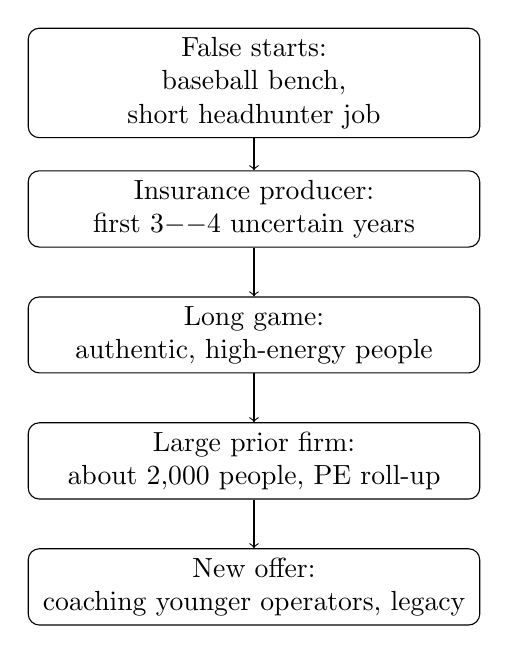
\begin{tikzpicture}[x=1cm,y=1cm]
\node[draw, rounded corners, align=center, text width=5.5cm] (a) at (0,0) {False starts:\\ baseball bench, short headhunter job};
\node[draw, rounded corners, align=center, text width=5.5cm] (b) at (0,-1.6) {Insurance producer:\\ first \(3\text{--}4\) uncertain years};
\node[draw, rounded corners, align=center, text width=5.5cm] (c) at (0,-3.2) {Long game:\\ authentic, high-energy people};
\node[draw, rounded corners, align=center, text width=5.5cm] (d) at (0,-4.8) {Large prior firm:\\ about \(2{,}000\) people, PE roll-up};
\node[draw, rounded corners, align=center, text width=5.5cm] (e) at (0,-6.4) {New offer:\\ coaching younger operators, legacy};
\draw[->] (a) -- (b);
\draw[->] (b) -- (c);
\draw[->] (c) -- (d);
\draw[->] (d) -- (e);
\end{tikzpicture}
\caption{A transcript-grounded career compounding ladder. The diagram is a reconstruction of the spoken sequence, not a screenshot-backed board figure.}
\end{figure}

\section{Luck, Timing, and Memory}

The interviewer next asks about Mike's best and worst financial decisions. The answers are useful because they separate three things that are often collapsed: good judgment, lucky timing, and personal meaning.

The best decision, Mike says, may have been Nautilus before the pandemic. He read about the company on an airplane roughly a month before the pandemic and noticed that it owned pieces of fitness-related brands such as Schwinn. He put money in, then put in more once it seemed that people stuck at home would buy exercise equipment. He calls the result pure luck.

The weaker decisions are Coinbase and the family home. Coinbase took back a lot of those winnings, though he was still holding. The family home is more subtle. He says they were there for more than twenty years and believes he may be the only person to stay in a house that long and break even. But he immediately adds that he would not trade the memories.

\begin{table}
\centering
\begin{tabular}{p{0.23\linewidth}p{0.32\linewidth}p{0.32\linewidth}}
\hline
Case & Financial reading & Personal or practical reading \\
\hline
Nautilus & Lucky timing before and during the pandemic & Acknowledged as luck, not a repeatable formula \\
Coinbase & Gave back some winnings & Still held with some hope \\
Family home & Roughly broke even after \(20+\) years & Preserved memories and family meaning \\
\hline
\end{tabular}
\caption{Mike's financial examples distinguish return, timing, and nonfinancial value.}
\end{table}

\subsection{Question \& Answer}

\paragraph{Question.}
Can a bad investment still be a good life decision?

\paragraph{Answer.}
In this interview, yes. The family home is named among the worst financial decisions because it apparently broke even after more than twenty years. But Mike refuses to treat the memories as worthless. The business lesson is not to ignore returns; it is to keep separate accounts: financial return in one column, family value in another.

\section{Analytics, Sales, and Specialization}

After the financial examples, the conversation circles back to industry choice. The older answer was private equity. In the 2023 framing of this interview, Mike adds data science and analytics. He is careful to say he is not an expert in the industry, but he sees analytics as important for insurance: younger people can crunch data and tell experienced operators what is trending.

The pivot from analytics to insurance sales is natural. If data tells us where patterns are forming, sales tests whether a firm can act on those patterns in front of a client. Mike's advice for insurance, and for sales more generally, is to avoid being alone on an island. He wants sales to feel like a team sport.

The concrete structure of the firm is numerical:
\begin{align}
N_{\text{sales people}} &\approx 25,\\
N_{\text{sales teams}} &\approx 5\text{--}6,\\
N_{\text{PE specialists}} &\approx 10,\\
N_{\text{restaurant clients}} &\approx 800.
\end{align}

These numbers support the mechanism. A generalist can talk about insurance. A specialist can talk about the client's world. Mike names private equity, hospitality, construction, and restaurants as verticals. The restaurant team, for example, can speak from hundreds of restaurant accounts and discuss retention problems, vendors, paving, or other practical headaches.

\begin{definition}
A \emph{vertical specialization} is a sales discipline organized around a client's industry rather than around a generic product pitch. In Mike's example, a producer who knows restaurants, hospitality, construction, or private equity can sell by recognizing the client's operating reality.
\end{definition}

The sales model can be written as an update rule for credibility. Let \(C_n\) denote credibility after \(n\) relevant client examples have been accumulated. A simple note-writing model is
\begin{equation}
C_{n+1}=C_n+\Delta_{\text{specificity}}+\Delta_{\text{trust}},
\end{equation}
where \(\Delta_{\text{specificity}}\) grows when the salesperson speaks concretely about the client's vertical, and \(\Delta_{\text{trust}}\) grows when the client believes the salesperson has seen similar problems before.

This is a reconstruction, but it is faithful to the interview: Mike's ``secret sauce'' is knowing how to talk the talk rather than remaining a generalist.

\begin{figure}
\centering
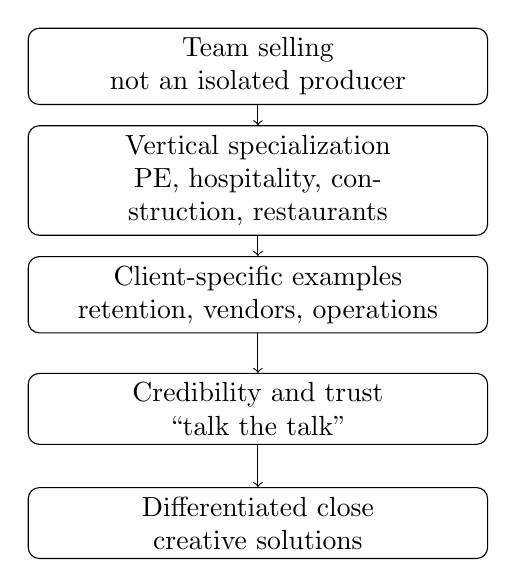
\begin{tikzpicture}[x=1cm,y=1cm]
\node[draw, rounded corners, align=center, text width=5.6cm] (a) at (0,0) {Team selling\\ not an isolated producer};
\node[draw, rounded corners, align=center, text width=5.6cm] (b) at (0,-1.45) {Vertical specialization\\ PE, hospitality, construction, restaurants};
\node[draw, rounded corners, align=center, text width=5.6cm] (c) at (0,-2.9) {Client-specific examples\\ retention, vendors, operations};
\node[draw, rounded corners, align=center, text width=5.6cm] (d) at (0,-4.35) {Credibility and trust\\ ``talk the talk''};
\node[draw, rounded corners, align=center, text width=5.6cm] (e) at (0,-5.8) {Differentiated close\\ creative solutions};
\draw[->] (a) -- (b);
\draw[->] (b) -- (c);
\draw[->] (c) -- (d);
\draw[->] (d) -- (e);
\end{tikzpicture}
\caption{The sales mechanism reconstructed from Mike's description of team selling and specialized verticals.}
\end{figure}

\section{The Personal Operating System}

The interview then shifts from business tactics to the operator behind the tactics. Mike names \emph{Don't Sweat the Small Stuff} as the book that most affected him, partly because it reminds him that most problems are not as large as they feel in the moment. He estimates that \(95\%\) of what happens is not really a big deal:
\begin{equation}
p_{\text{not a big deal}}\approx 0.95.
\end{equation}

The family section preserves another operating principle. For children, Mike emphasizes quantity of time, especially when they are young. For marriage, he says the person who has been a ``hammer'' at work may need to pause before entering the house, take a breath, and remember to be a partner. He also stresses affection, humor, and common interests.

Then the interviewer asks about daily habits. Mike says he is working harder than ever, but it does not feel like work because he is surrounded by energetic younger people. His morning routine begins with a triple espresso in what he calls his parlor, then a few minutes of meditation and gratitude toward his family, his work, Austin, and being away from Chicago weather.

The durations are modest:
\begin{align}
t_{\text{gratitude}} &\approx 30\ \text{seconds}\text{--}5\ \text{minutes},\\
t_{\text{meditation}} &\approx 3\ \text{minutes}\quad\text{or}\quad 8\ \text{minutes}.
\end{align}

\subsection{Question \& Answer}

\paragraph{Question.}
Do habits like gratitude and meditation actually affect business performance, or are they just slogans?

\paragraph{Answer.}
Mike's answer is deliberately unsentimental. He says the espresso is the best part; gratitude is easy because everyone has something to be thankful for; and meditation often includes thoughts about business or family. But the habit still matters because he feels good when he is done. The mechanism is not mystical. It is an opening routine that stabilizes attention before the workday begins.

\section{Plan, Tenacity, and the Zero-Bank-Account Test}

The next question asks for the mindset change required to become a multimillionaire. Mike answers in two parts: first, actually come up with a plan; second, have the tenacity and wherewithal to execute it. He adds that many people give up a day, a week, or a month before the business might have broken through.

We can write this as a minimal execution inequality. Let \(R(t)\) be the resources remaining at time \(t\), and let \(B(t)\) be the required burden of continuing. A venture survives one more period only if
\begin{equation}
R(t) \geq B(t).
\end{equation}
Mike's point is qualitative: people often stop just before the reward function changes. The plan matters, but so does the staying power to keep \(R(t)\) above the burden long enough for opportunity to appear.

When the interviewer asks what he would do if his bank account hit zero, Mike gives the most direct recovery mechanism in the interview. He would return to full-time sales because he believes he could still hustle, outwork others, and generate commission checks quickly. Then he would redeploy those checks into real estate, private companies or private equity, and possibly hobbies that can become financially successful.

\begin{enumerate}
\item Return to full-time sales.
\item Generate commission cash flow quickly.
\item Allocate the cash flow into assets or ownership opportunities.
\item Rebuild optionality through real estate, private companies, or commercialized hobbies.
\end{enumerate}

In compact form:
\begin{equation}
\text{full-time sales}
\longrightarrow
\text{commission cash flow}
\longrightarrow
\text{ownership assets}
\longrightarrow
\text{rebuilt optionality}.
\end{equation}

\begin{figure}
\centering
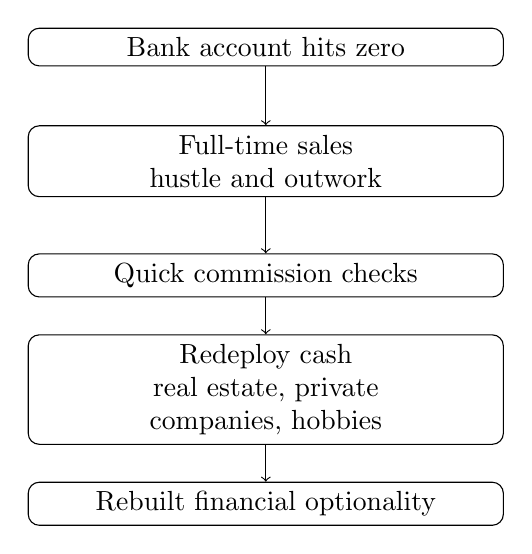
\begin{tikzpicture}[x=1cm,y=1cm]
\node[draw, rounded corners, align=center, text width=5.8cm] (a) at (0,0) {Bank account hits zero};
\node[draw, rounded corners, align=center, text width=5.8cm] (b) at (0,-1.45) {Full-time sales\\ hustle and outwork};
\node[draw, rounded corners, align=center, text width=5.8cm] (c) at (0,-2.9) {Quick commission checks};
\node[draw, rounded corners, align=center, text width=5.8cm] (d) at (0,-4.35) {Redeploy cash\\ real estate, private companies, hobbies};
\node[draw, rounded corners, align=center, text width=5.8cm] (e) at (0,-5.8) {Rebuilt financial optionality};
\draw[->] (a) -- (b);
\draw[->] (b) -- (c);
\draw[->] (c) -- (d);
\draw[->] (d) -- (e);
\end{tikzpicture}
\caption{The rebuilding sequence as Mike gives it: earn first through sales, then redeploy into ownership-like assets.}
\end{figure}

\subsection{Question \& Answer}

\paragraph{Question.}
What survives if the money disappears?

\paragraph{Answer.}
For Mike, the durable asset is not the bank balance. It is the ability to sell, work, and turn effort into cash flow. Once cash flow returns, the investment menu reopens. In this interview, sales is the first engine because it can be restarted faster than a large balance sheet.

\section{Virtus and the Legacy Claim}

Near the end, the interviewer asks how Mike wants to be remembered. Mike answers with family first: honorable, hard-working, a strong husband and father, authentic and real. He also wants to be remembered as someone who performed forcefully in business. The phrasing is blunt, but the structure is consistent with the rest of the interview: family foundation first, commercial drive second.

He then describes Virtus. The firm is headquartered in Kansas City, with offices in Fort Collins, Chicago, St. Louis, Austin, Fort Worth, and Memphis. Mike says the firm has over one hundred people and positions itself against an insurance industry he describes as slow, old, and stale.

\begin{equation}
N_{\text{Virtus people}} > 100.
\end{equation}

The growth claim is also important:
\begin{equation}
G_{\text{Virtus}} \approx 4 \quad \text{over} \quad 3\ \text{years}.
\end{equation}
Mike says the firm has quadrupled in three years. He frames his present motivation as legacy: having a small impact on younger men and women who may go on to make millions of dollars and, more importantly, become better professionally and personally.

\begin{proposition}
In Mike's account, durable wealth is not only accumulated capital. It is a combination of cash-flow skill, trusted relationships, specialized knowledge, and enough freedom to choose one's next room.
\end{proposition}

\begin{proof}
The transcript supplies each part separately. Cash-flow skill appears in the zero-bank-account answer: return to full-time sales and generate commissions. Trusted relationships appear in the long-game story that leads to the later offer. Specialized knowledge appears in the vertical sales teams. Freedom appears in Mike's definition of success: being able to breathe, pay the bills, leave bad people, get another job, or start one's own path. These pieces do not form a theorem in the mathematical sense, but they do form the interview's operating logic.
\end{proof}

\section{Summary}

Mike Kessner's interview begins with private equity, but it does not stay there. The deeper pattern is a career built through false starts, long-duration relationships, team selling, vertical specialization, and the ability to rebuild cash flow through sales. The quantitative anchors are modest but concrete: more than thirty years in insurance, three or four uncertain early years, more than twenty-five years playing the long game, a prior firm of about two thousand people, roughly twenty-five sales people across five or six teams, about ten private-equity specialists, roughly eight hundred restaurant clients, and a firm that Mike says quadrupled in three years.

For the dynamic book, this interview should feed several durable questions rather than stand as a single isolated chapter. It contributes to the chapters on industry choice, relationships, sales skill, risk recovery, operating discipline, family, legacy, and what wealth is for after the number is reached.